\documentclass{article} % For LaTeX2e
\usepackage{iclr2021_conference,times}
\usepackage{ltablex}
\usepackage{listings}
%%%%% NEW MATH DEFINITIONS %%%%%

\usepackage{amsmath,amsfonts,bm}

% Mark sections of captions for referring to divisions of figures
\newcommand{\figleft}{{\em (Left)}}
\newcommand{\figcenter}{{\em (Center)}}
\newcommand{\figright}{{\em (Right)}}
\newcommand{\figtop}{{\em (Top)}}
\newcommand{\figbottom}{{\em (Bottom)}}
\newcommand{\captiona}{{\em (a)}}
\newcommand{\captionb}{{\em (b)}}
\newcommand{\captionc}{{\em (c)}}
\newcommand{\captiond}{{\em (d)}}

% Highlight a newly defined term
\newcommand{\newterm}[1]{{\bf #1}}


% Figure reference, lower-case.
\def\figref#1{figure~\ref{#1}}
% Figure reference, capital. For start of sentence
\def\Figref#1{Figure~\ref{#1}}
\def\twofigref#1#2{figures \ref{#1} and \ref{#2}}
\def\quadfigref#1#2#3#4{figures \ref{#1}, \ref{#2}, \ref{#3} and \ref{#4}}
% Section reference, lower-case.
\def\secref#1{section~\ref{#1}}
% Section reference, capital.
\def\Secref#1{Section~\ref{#1}}
% Reference to two sections.
\def\twosecrefs#1#2{sections \ref{#1} and \ref{#2}}
% Reference to three sections.
\def\secrefs#1#2#3{sections \ref{#1}, \ref{#2} and \ref{#3}}
% Reference to an equation, lower-case.
\def\eqref#1{equation~\ref{#1}}
% Reference to an equation, upper case
\def\Eqref#1{Equation~\ref{#1}}
% A raw reference to an equation---avoid using if possible
\def\plaineqref#1{\ref{#1}}
% Reference to a chapter, lower-case.
\def\chapref#1{chapter~\ref{#1}}
% Reference to an equation, upper case.
\def\Chapref#1{Chapter~\ref{#1}}
% Reference to a range of chapters
\def\rangechapref#1#2{chapters\ref{#1}--\ref{#2}}
% Reference to an algorithm, lower-case.
\def\algref#1{algorithm~\ref{#1}}
% Reference to an algorithm, upper case.
\def\Algref#1{Algorithm~\ref{#1}}
\def\twoalgref#1#2{algorithms \ref{#1} and \ref{#2}}
\def\Twoalgref#1#2{Algorithms \ref{#1} and \ref{#2}}
% Reference to a part, lower case
\def\partref#1{part~\ref{#1}}
% Reference to a part, upper case
\def\Partref#1{Part~\ref{#1}}
\def\twopartref#1#2{parts \ref{#1} and \ref{#2}}

\def\ceil#1{\lceil #1 \rceil}
\def\floor#1{\lfloor #1 \rfloor}
\def\1{\bm{1}}
\newcommand{\train}{\mathcal{D}}
\newcommand{\valid}{\mathcal{D_{\mathrm{valid}}}}
\newcommand{\test}{\mathcal{D_{\mathrm{test}}}}

\def\eps{{\epsilon}}


% Random variables
\def\reta{{\textnormal{$\eta$}}}
\def\ra{{\textnormal{a}}}
\def\rb{{\textnormal{b}}}
\def\rc{{\textnormal{c}}}
\def\rd{{\textnormal{d}}}
\def\re{{\textnormal{e}}}
\def\rf{{\textnormal{f}}}
\def\rg{{\textnormal{g}}}
\def\rh{{\textnormal{h}}}
\def\ri{{\textnormal{i}}}
\def\rj{{\textnormal{j}}}
\def\rk{{\textnormal{k}}}
\def\rl{{\textnormal{l}}}
% rm is already a command, just don't name any random variables m
\def\rn{{\textnormal{n}}}
\def\ro{{\textnormal{o}}}
\def\rp{{\textnormal{p}}}
\def\rq{{\textnormal{q}}}
\def\rr{{\textnormal{r}}}
\def\rs{{\textnormal{s}}}
\def\rt{{\textnormal{t}}}
\def\ru{{\textnormal{u}}}
\def\rv{{\textnormal{v}}}
\def\rw{{\textnormal{w}}}
\def\rx{{\textnormal{x}}}
\def\ry{{\textnormal{y}}}
\def\rz{{\textnormal{z}}}

% Random vectors
\def\rvepsilon{{\mathbf{\epsilon}}}
\def\rvtheta{{\mathbf{\theta}}}
\def\rva{{\mathbf{a}}}
\def\rvb{{\mathbf{b}}}
\def\rvc{{\mathbf{c}}}
\def\rvd{{\mathbf{d}}}
\def\rve{{\mathbf{e}}}
\def\rvf{{\mathbf{f}}}
\def\rvg{{\mathbf{g}}}
\def\rvh{{\mathbf{h}}}
\def\rvu{{\mathbf{i}}}
\def\rvj{{\mathbf{j}}}
\def\rvk{{\mathbf{k}}}
\def\rvl{{\mathbf{l}}}
\def\rvm{{\mathbf{m}}}
\def\rvn{{\mathbf{n}}}
\def\rvo{{\mathbf{o}}}
\def\rvp{{\mathbf{p}}}
\def\rvq{{\mathbf{q}}}
\def\rvr{{\mathbf{r}}}
\def\rvs{{\mathbf{s}}}
\def\rvt{{\mathbf{t}}}
\def\rvu{{\mathbf{u}}}
\def\rvv{{\mathbf{v}}}
\def\rvw{{\mathbf{w}}}
\def\rvx{{\mathbf{x}}}
\def\rvy{{\mathbf{y}}}
\def\rvz{{\mathbf{z}}}

% Elements of random vectors
\def\erva{{\textnormal{a}}}
\def\ervb{{\textnormal{b}}}
\def\ervc{{\textnormal{c}}}
\def\ervd{{\textnormal{d}}}
\def\erve{{\textnormal{e}}}
\def\ervf{{\textnormal{f}}}
\def\ervg{{\textnormal{g}}}
\def\ervh{{\textnormal{h}}}
\def\ervi{{\textnormal{i}}}
\def\ervj{{\textnormal{j}}}
\def\ervk{{\textnormal{k}}}
\def\ervl{{\textnormal{l}}}
\def\ervm{{\textnormal{m}}}
\def\ervn{{\textnormal{n}}}
\def\ervo{{\textnormal{o}}}
\def\ervp{{\textnormal{p}}}
\def\ervq{{\textnormal{q}}}
\def\ervr{{\textnormal{r}}}
\def\ervs{{\textnormal{s}}}
\def\ervt{{\textnormal{t}}}
\def\ervu{{\textnormal{u}}}
\def\ervv{{\textnormal{v}}}
\def\ervw{{\textnormal{w}}}
\def\ervx{{\textnormal{x}}}
\def\ervy{{\textnormal{y}}}
\def\ervz{{\textnormal{z}}}

% Random matrices
\def\rmA{{\mathbf{A}}}
\def\rmB{{\mathbf{B}}}
\def\rmC{{\mathbf{C}}}
\def\rmD{{\mathbf{D}}}
\def\rmE{{\mathbf{E}}}
\def\rmF{{\mathbf{F}}}
\def\rmG{{\mathbf{G}}}
\def\rmH{{\mathbf{H}}}
\def\rmI{{\mathbf{I}}}
\def\rmJ{{\mathbf{J}}}
\def\rmK{{\mathbf{K}}}
\def\rmL{{\mathbf{L}}}
\def\rmM{{\mathbf{M}}}
\def\rmN{{\mathbf{N}}}
\def\rmO{{\mathbf{O}}}
\def\rmP{{\mathbf{P}}}
\def\rmQ{{\mathbf{Q}}}
\def\rmR{{\mathbf{R}}}
\def\rmS{{\mathbf{S}}}
\def\rmT{{\mathbf{T}}}
\def\rmU{{\mathbf{U}}}
\def\rmV{{\mathbf{V}}}
\def\rmW{{\mathbf{W}}}
\def\rmX{{\mathbf{X}}}
\def\rmY{{\mathbf{Y}}}
\def\rmZ{{\mathbf{Z}}}

% Elements of random matrices
\def\ermA{{\textnormal{A}}}
\def\ermB{{\textnormal{B}}}
\def\ermC{{\textnormal{C}}}
\def\ermD{{\textnormal{D}}}
\def\ermE{{\textnormal{E}}}
\def\ermF{{\textnormal{F}}}
\def\ermG{{\textnormal{G}}}
\def\ermH{{\textnormal{H}}}
\def\ermI{{\textnormal{I}}}
\def\ermJ{{\textnormal{J}}}
\def\ermK{{\textnormal{K}}}
\def\ermL{{\textnormal{L}}}
\def\ermM{{\textnormal{M}}}
\def\ermN{{\textnormal{N}}}
\def\ermO{{\textnormal{O}}}
\def\ermP{{\textnormal{P}}}
\def\ermQ{{\textnormal{Q}}}
\def\ermR{{\textnormal{R}}}
\def\ermS{{\textnormal{S}}}
\def\ermT{{\textnormal{T}}}
\def\ermU{{\textnormal{U}}}
\def\ermV{{\textnormal{V}}}
\def\ermW{{\textnormal{W}}}
\def\ermX{{\textnormal{X}}}
\def\ermY{{\textnormal{Y}}}
\def\ermZ{{\textnormal{Z}}}

% Vectors
\def\vzero{{\bm{0}}}
\def\vone{{\bm{1}}}
\def\vmu{{\bm{\mu}}}
\def\vtheta{{\bm{\theta}}}
\def\va{{\bm{a}}}
\def\vb{{\bm{b}}}
\def\vc{{\bm{c}}}
\def\vd{{\bm{d}}}
\def\ve{{\bm{e}}}
\def\vf{{\bm{f}}}
\def\vg{{\bm{g}}}
\def\vh{{\bm{h}}}
\def\vi{{\bm{i}}}
\def\vj{{\bm{j}}}
\def\vk{{\bm{k}}}
\def\vl{{\bm{l}}}
\def\vm{{\bm{m}}}
\def\vn{{\bm{n}}}
\def\vo{{\bm{o}}}
\def\vp{{\bm{p}}}
\def\vq{{\bm{q}}}
\def\vr{{\bm{r}}}
\def\vs{{\bm{s}}}
\def\vt{{\bm{t}}}
\def\vu{{\bm{u}}}
\def\vv{{\bm{v}}}
\def\vw{{\bm{w}}}
\def\vx{{\bm{x}}}
\def\vy{{\bm{y}}}
\def\vz{{\bm{z}}}

% Elements of vectors
\def\evalpha{{\alpha}}
\def\evbeta{{\beta}}
\def\evepsilon{{\epsilon}}
\def\evlambda{{\lambda}}
\def\evomega{{\omega}}
\def\evmu{{\mu}}
\def\evpsi{{\psi}}
\def\evsigma{{\sigma}}
\def\evtheta{{\theta}}
\def\eva{{a}}
\def\evb{{b}}
\def\evc{{c}}
\def\evd{{d}}
\def\eve{{e}}
\def\evf{{f}}
\def\evg{{g}}
\def\evh{{h}}
\def\evi{{i}}
\def\evj{{j}}
\def\evk{{k}}
\def\evl{{l}}
\def\evm{{m}}
\def\evn{{n}}
\def\evo{{o}}
\def\evp{{p}}
\def\evq{{q}}
\def\evr{{r}}
\def\evs{{s}}
\def\evt{{t}}
\def\evu{{u}}
\def\evv{{v}}
\def\evw{{w}}
\def\evx{{x}}
\def\evy{{y}}
\def\evz{{z}}

% Matrix
\def\mA{{\bm{A}}}
\def\mB{{\bm{B}}}
\def\mC{{\bm{C}}}
\def\mD{{\bm{D}}}
\def\mE{{\bm{E}}}
\def\mF{{\bm{F}}}
\def\mG{{\bm{G}}}
\def\mH{{\bm{H}}}
\def\mI{{\bm{I}}}
\def\mJ{{\bm{J}}}
\def\mK{{\bm{K}}}
\def\mL{{\bm{L}}}
\def\mM{{\bm{M}}}
\def\mN{{\bm{N}}}
\def\mO{{\bm{O}}}
\def\mP{{\bm{P}}}
\def\mQ{{\bm{Q}}}
\def\mR{{\bm{R}}}
\def\mS{{\bm{S}}}
\def\mT{{\bm{T}}}
\def\mU{{\bm{U}}}
\def\mV{{\bm{V}}}
\def\mW{{\bm{W}}}
\def\mX{{\bm{X}}}
\def\mY{{\bm{Y}}}
\def\mZ{{\bm{Z}}}
\def\mBeta{{\bm{\beta}}}
\def\mPhi{{\bm{\Phi}}}
\def\mLambda{{\bm{\Lambda}}}
\def\mSigma{{\bm{\Sigma}}}

% Tensor
\DeclareMathAlphabet{\mathsfit}{\encodingdefault}{\sfdefault}{m}{sl}
\SetMathAlphabet{\mathsfit}{bold}{\encodingdefault}{\sfdefault}{bx}{n}
\newcommand{\tens}[1]{\bm{\mathsfit{#1}}}
\def\tA{{\tens{A}}}
\def\tB{{\tens{B}}}
\def\tC{{\tens{C}}}
\def\tD{{\tens{D}}}
\def\tE{{\tens{E}}}
\def\tF{{\tens{F}}}
\def\tG{{\tens{G}}}
\def\tH{{\tens{H}}}
\def\tI{{\tens{I}}}
\def\tJ{{\tens{J}}}
\def\tK{{\tens{K}}}
\def\tL{{\tens{L}}}
\def\tM{{\tens{M}}}
\def\tN{{\tens{N}}}
\def\tO{{\tens{O}}}
\def\tP{{\tens{P}}}
\def\tQ{{\tens{Q}}}
\def\tR{{\tens{R}}}
\def\tS{{\tens{S}}}
\def\tT{{\tens{T}}}
\def\tU{{\tens{U}}}
\def\tV{{\tens{V}}}
\def\tW{{\tens{W}}}
\def\tX{{\tens{X}}}
\def\tY{{\tens{Y}}}
\def\tZ{{\tens{Z}}}


% Graph
\def\gA{{\mathcal{A}}}
\def\gB{{\mathcal{B}}}
\def\gC{{\mathcal{C}}}
\def\gD{{\mathcal{D}}}
\def\gE{{\mathcal{E}}}
\def\gF{{\mathcal{F}}}
\def\gG{{\mathcal{G}}}
\def\gH{{\mathcal{H}}}
\def\gI{{\mathcal{I}}}
\def\gJ{{\mathcal{J}}}
\def\gK{{\mathcal{K}}}
\def\gL{{\mathcal{L}}}
\def\gM{{\mathcal{M}}}
\def\gN{{\mathcal{N}}}
\def\gO{{\mathcal{O}}}
\def\gP{{\mathcal{P}}}
\def\gQ{{\mathcal{Q}}}
\def\gR{{\mathcal{R}}}
\def\gS{{\mathcal{S}}}
\def\gT{{\mathcal{T}}}
\def\gU{{\mathcal{U}}}
\def\gV{{\mathcal{V}}}
\def\gW{{\mathcal{W}}}
\def\gX{{\mathcal{X}}}
\def\gY{{\mathcal{Y}}}
\def\gZ{{\mathcal{Z}}}

% Sets
\def\sA{{\mathbb{A}}}
\def\sB{{\mathbb{B}}}
\def\sC{{\mathbb{C}}}
\def\sD{{\mathbb{D}}}
% Don't use a set called E, because this would be the same as our symbol
% for expectation.
\def\sF{{\mathbb{F}}}
\def\sG{{\mathbb{G}}}
\def\sH{{\mathbb{H}}}
\def\sI{{\mathbb{I}}}
\def\sJ{{\mathbb{J}}}
\def\sK{{\mathbb{K}}}
\def\sL{{\mathbb{L}}}
\def\sM{{\mathbb{M}}}
\def\sN{{\mathbb{N}}}
\def\sO{{\mathbb{O}}}
\def\sP{{\mathbb{P}}}
\def\sQ{{\mathbb{Q}}}
\def\sR{{\mathbb{R}}}
\def\sS{{\mathbb{S}}}
\def\sT{{\mathbb{T}}}
\def\sU{{\mathbb{U}}}
\def\sV{{\mathbb{V}}}
\def\sW{{\mathbb{W}}}
\def\sX{{\mathbb{X}}}
\def\sY{{\mathbb{Y}}}
\def\sZ{{\mathbb{Z}}}

% Entries of a matrix
\def\emLambda{{\Lambda}}
\def\emA{{A}}
\def\emB{{B}}
\def\emC{{C}}
\def\emD{{D}}
\def\emE{{E}}
\def\emF{{F}}
\def\emG{{G}}
\def\emH{{H}}
\def\emI{{I}}
\def\emJ{{J}}
\def\emK{{K}}
\def\emL{{L}}
\def\emM{{M}}
\def\emN{{N}}
\def\emO{{O}}
\def\emP{{P}}
\def\emQ{{Q}}
\def\emR{{R}}
\def\emS{{S}}
\def\emT{{T}}
\def\emU{{U}}
\def\emV{{V}}
\def\emW{{W}}
\def\emX{{X}}
\def\emY{{Y}}
\def\emZ{{Z}}
\def\emSigma{{\Sigma}}

% entries of a tensor
% Same font as tensor, without \bm wrapper
\newcommand{\etens}[1]{\mathsfit{#1}}
\def\etLambda{{\etens{\Lambda}}}
\def\etA{{\etens{A}}}
\def\etB{{\etens{B}}}
\def\etC{{\etens{C}}}
\def\etD{{\etens{D}}}
\def\etE{{\etens{E}}}
\def\etF{{\etens{F}}}
\def\etG{{\etens{G}}}
\def\etH{{\etens{H}}}
\def\etI{{\etens{I}}}
\def\etJ{{\etens{J}}}
\def\etK{{\etens{K}}}
\def\etL{{\etens{L}}}
\def\etM{{\etens{M}}}
\def\etN{{\etens{N}}}
\def\etO{{\etens{O}}}
\def\etP{{\etens{P}}}
\def\etQ{{\etens{Q}}}
\def\etR{{\etens{R}}}
\def\etS{{\etens{S}}}
\def\etT{{\etens{T}}}
\def\etU{{\etens{U}}}
\def\etV{{\etens{V}}}
\def\etW{{\etens{W}}}
\def\etX{{\etens{X}}}
\def\etY{{\etens{Y}}}
\def\etZ{{\etens{Z}}}

% The true underlying data generating distribution
\newcommand{\pdata}{p_{\rm{data}}}
% The empirical distribution defined by the training set
\newcommand{\ptrain}{\hat{p}_{\rm{data}}}
\newcommand{\Ptrain}{\hat{P}_{\rm{data}}}
% The model distribution
\newcommand{\pmodel}{p_{\rm{model}}}
\newcommand{\Pmodel}{P_{\rm{model}}}
\newcommand{\ptildemodel}{\tilde{p}_{\rm{model}}}
% Stochastic autoencoder distributions
\newcommand{\pencode}{p_{\rm{encoder}}}
\newcommand{\pdecode}{p_{\rm{decoder}}}
\newcommand{\precons}{p_{\rm{reconstruct}}}

\newcommand{\laplace}{\mathrm{Laplace}} % Laplace distribution

\newcommand{\E}{\mathbb{E}}
\newcommand{\Ls}{\mathcal{L}}
\newcommand{\R}{\mathbb{R}}
\newcommand{\emp}{\tilde{p}}
\newcommand{\lr}{\alpha}
\newcommand{\reg}{\lambda}
\newcommand{\rect}{\mathrm{rectifier}}
\newcommand{\softmax}{\mathrm{softmax}}
\newcommand{\sigmoid}{\sigma}
\newcommand{\softplus}{\zeta}
\newcommand{\KL}{D_{\mathrm{KL}}}
\newcommand{\Var}{\mathrm{Var}}
\newcommand{\standarderror}{\mathrm{SE}}
\newcommand{\Cov}{\mathrm{Cov}}
% Wolfram Mathworld says $L^2$ is for function spaces and $\ell^2$ is for vectors
% But then they seem to use $L^2$ for vectors throughout the site, and so does
% wikipedia.
\newcommand{\normlzero}{L^0}
\newcommand{\normlone}{L^1}
\newcommand{\normltwo}{L^2}
\newcommand{\normlp}{L^p}
\newcommand{\normmax}{L^\infty}

\newcommand{\parents}{Pa} % See usage in notation.tex. Chosen to match Daphne's book.

\DeclareMathOperator*{\argmax}{arg\,max}
\DeclareMathOperator*{\argmin}{arg\,min}

\DeclareMathOperator{\sign}{sign}
\DeclareMathOperator{\Tr}{Tr}
\let\ab\allowbreak

\usepackage{float}
\usepackage{hyperref}
\usepackage{url}
\usepackage{graphicx}
\usepackage{multirow}
\graphicspath{ {./images/} }

\title{Computer Vision Evaluation \\ Report on the FaceForensics++ paper}

% Authors must not appear in the submitted version. They should be hidden
% as long as the \iclrfinalcopy macro remains commented out below.
% Non-anonymous submissions will be rejected without review.

\author{Quentin Le Roux \\
MSc in Data Science \& Artificial Intelligence \\
Université Côte d'Azur \\
\texttt{quentin.leroux@edhec.com}}

% The \author macro works with any number of authors. There are two commands
% used to separate the names and addresses of multiple authors: \And and \AND.
%
% Using \And between authors leaves it to \LaTeX{} to determine where to break
% the lines. Using \AND forces a linebreak at that point. So, if \LaTeX{}
% puts 3 of 4 authors names on the first line, and the last on the second
% line, try using \AND instead of \And before the third author name.

\newcommand{\fix}{\marginpar{FIX}}
\newcommand{\new}{\marginpar{NEW}}

\iclrfinalcopy % Uncomment for camera-ready version, but NOT for submission.
\begin{document}

\begin{center}
\maketitle
\end{center}

\begin{abstract}
FaceForensics++ is a seminal paper in computer vision and specifically facial forgery detection. The present report offers an overview of the paper, and the namesake dataset it was published with, as well as a re-implementation of its best model based on the XceptionNet architecture. We also cover more recent developments as well as try to outperform its results.
\end{abstract}

\section{Introduction}

Image manipulation is an old field of research with roots hearkening back to the the birth of photography itself. One of the earliest and most well-known image manipulations is that of US President Abraham Lincoln's lithography portrait where the US politician John Calhoun body's was doctored in to replace his (See Figure 1).

\begin{figure}[H]
\begin{center}
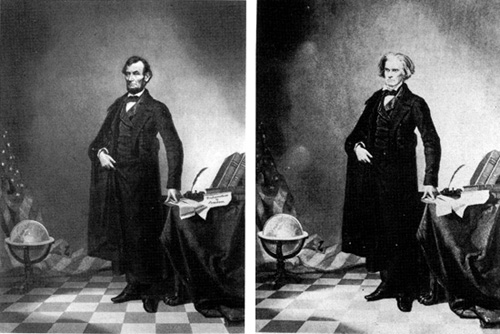
\includegraphics[width=0.6\textwidth]{images/lincoln_manip.jpg}
\end{center}
\caption{Lithography manipulation of US President A. Lincoln circa 1860 \citep{PRI}}
\end{figure}

Over the past decade, the field of computer vision underwent a revolution with the development of new methods thanks to Deep Learning. The computational barrier to entry of image detection as well as manipulation lowered, making such models and methods ubiquitous both as products and a tools. This has raised concerns, however, notably with regards to their potential social, political, and economic impact. The paper notes loss of trust and broader harm to society as an example risk \citep{DBLP:journals/corr/abs-1803-09179}. 

The paper outlines two main types of image manipulations, specifically regarding facial features \citep{DBLP:journals/corr/abs-1803-09179}:
\begin{itemize}
    \item Expression manipulation
    \item Identity manipulation
\end{itemize}
Expression manipulation targets the modification of facial expressions, or their transfer between two persons. Meanwhile, identity manipulation aims at replacing a face entirely either by pasting over, replacing, or replicating another. 

Those two types of methods can be applied to images or videos \citep{DBLP:journals/corr/KorshunovaSDT16}. As such, the reliable and automatic detection of forgeries (the paper specifically mentions the DeepFakes  project\citep{faceswap}) has become a prominent area of research as newer doctoring methods must be met with more efficient detection models.

\section{The state-of-the-art at the time of publication (October 2019)}

\subsection{Forgery methods}

Face manipulation techniques can be broadly sorted into two families (See Table 1). The oldest relies on non deep-learning methods while the other, more recent, group of techniques heavily relies on Generative Adversarial Networks.

\begin{table}[h!]
\centering
\begin{tabular}{ |p{3cm}|p{5.5cm}|p{4cm}|  }
 \hline
 \multicolumn{3}{|c|}{Non deep-learning face manipulation methods} \\
 \hline
 \textbf{Type} & \textbf{Name or use} & \textbf{Papers} \\
 \hline
 Video generation & Video Rewrite & \cite{8014966} \\
 Face replacement & Video Face Replacement & \cite{dale2011video} \\
  & VDub & \cite{10.1111/cgf.12552} \\
  & Real-time expression transfer for facial reenactment & \cite{10.1145/2816795.2818056} \\
  & Face2Face & \cite{Thies2018Face2Face} \\
 Virtual Reality & FaceVR & \cite{10.1145/3182644} \\
  & Headon & \cite{Thies_2018} \\
 Reenactment & Deep Video Portraits & \cite{kim2018deep} \\
  & NeuralTextures & \cite{thies2019deferred} \\
  & Bringing Portraits To Life & \cite{elor2017bringingPortraits} \\
 Audio-video syncing & Synthesizing Obama & \cite{10.1145/3072959.3073640} \\
 & & \\
 \hline
 \multicolumn{3}{|c|}{Deep-learning face manipulation methods} \\
 \hline
 \textbf{Type} & \textbf{Name or use} & \textbf{Papers} \\
 \hline
 GANs & Face Aging & \cite{antipov2017face} \\
  & Frontal View Synthesis & \cite{8237529} \\
  & Face attribute alteration & \cite{article} \\
  & Deep Feature Interpolation & \cite{upchurch2017deep} \\
 Fader Networks & Fader Networks & \cite{lample2018fader} \\
 \hline
\end{tabular}
\caption{State-of-the-art of face manipulation techniques}
\end{table}

\subsubsection{Graphics-based methods: Face2Face}

Non deep-learning methods rely on first tracking the location of a face in two monocular videos (i.e. there are no editing cuts, the video is a single shot without change of angle): the source and target videos. Once the face tracking model is at play, a face transfer model of the tracked features is performed.

Such a method type is exemplified by the Face2Face process \citep{Thies2018Face2Face}, one of the main sources of data of the paper at hand here. 

\begin{figure}[H]
\begin{center}
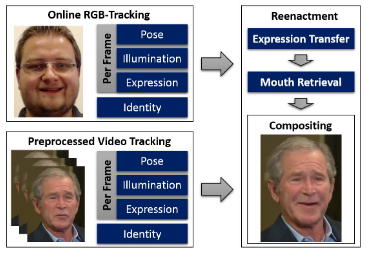
\includegraphics[width=0.5\textwidth]{images/method.png}
\end{center}
\caption{Method of the Face2Face algorithm \citep{Thies2018Face2Face}}
\end{figure}

Face2Face relies on a so-called parametric face model, (a parameter vector $P$, see Figure 3, that captures the rigid pose of the face (6 degrees of freedom), its shape (80 dof), its albedo/identity (80 dof), its expression (76 dof), and its illumination (27 dof), totalling 269 parameters).

\begin{figure}[H]
\begin{center}
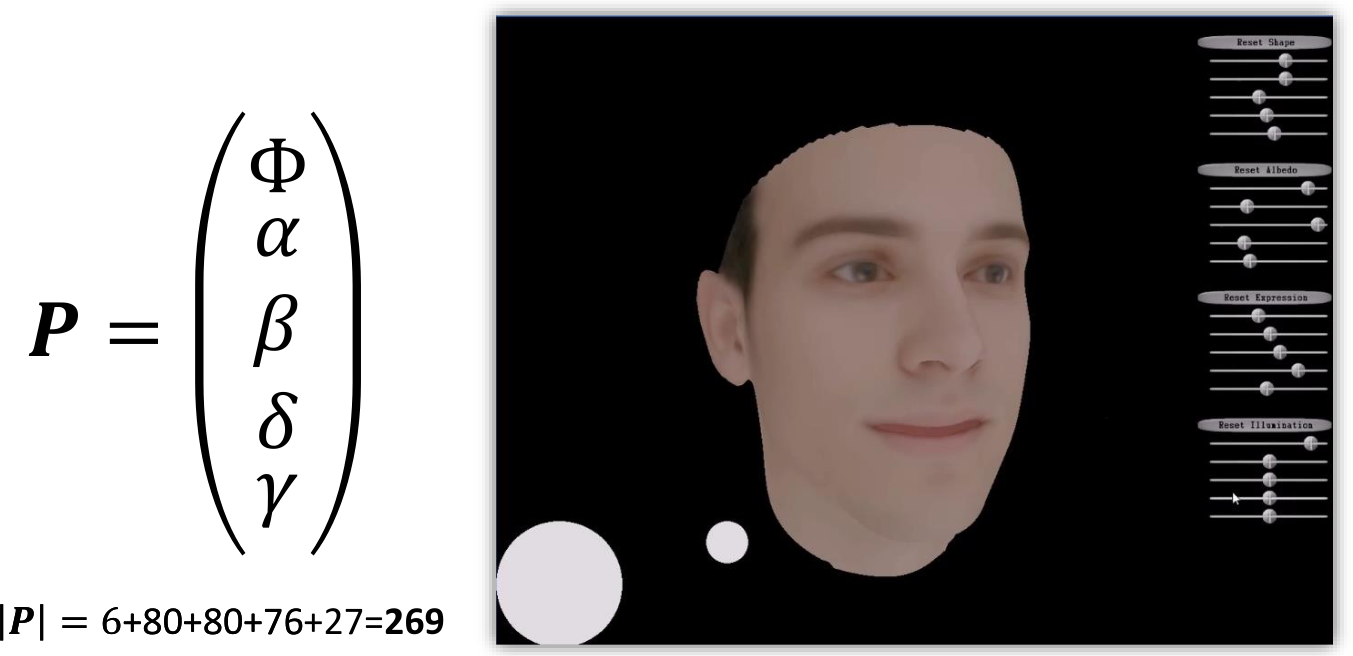
\includegraphics[width=0.5\textwidth]{images/parametric.png}
\end{center}
\caption{Parametric face model of the Face2Face method \citep{Thies2016}}
\end{figure}

The process relies on graphics card processing to model/rasterize the image and perform a face capture from a source and target videos. Face capture relies on an energy formulation per frame (see Figure 4) that estimates the different parameters of the face to be modified, smoothed over several keyframes using a technique called non-rigid model-based bundling (see Figure 5), which relies on iterative reweighted least squares. The end result is the capture of the geometry and texture of a person's face and the ability to track its movement throughout a video.

\begin{figure}[H]
\begin{center}
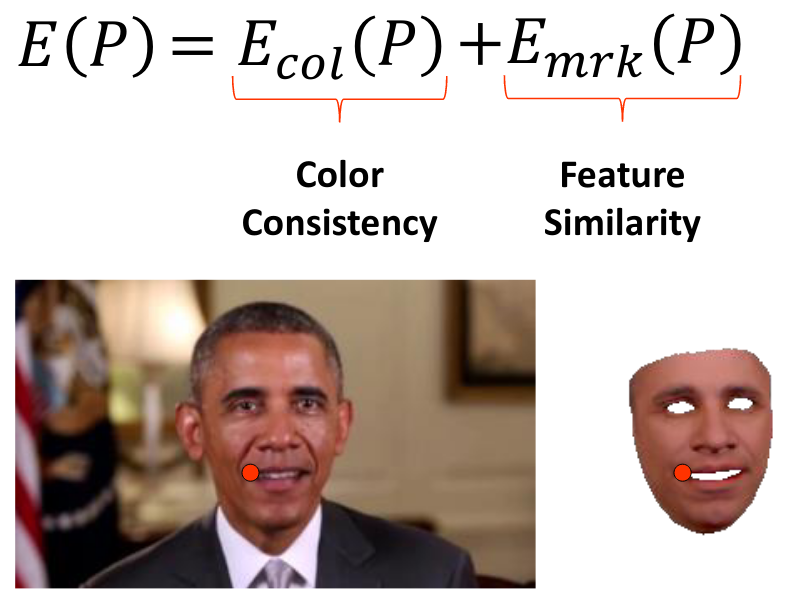
\includegraphics[width=0.5\textwidth]{images/energy.png}
\end{center}
\caption{Energy formulation of the Face2Face method \citep{Thies2016}}
\end{figure}

\begin{figure}[H]
\begin{center}
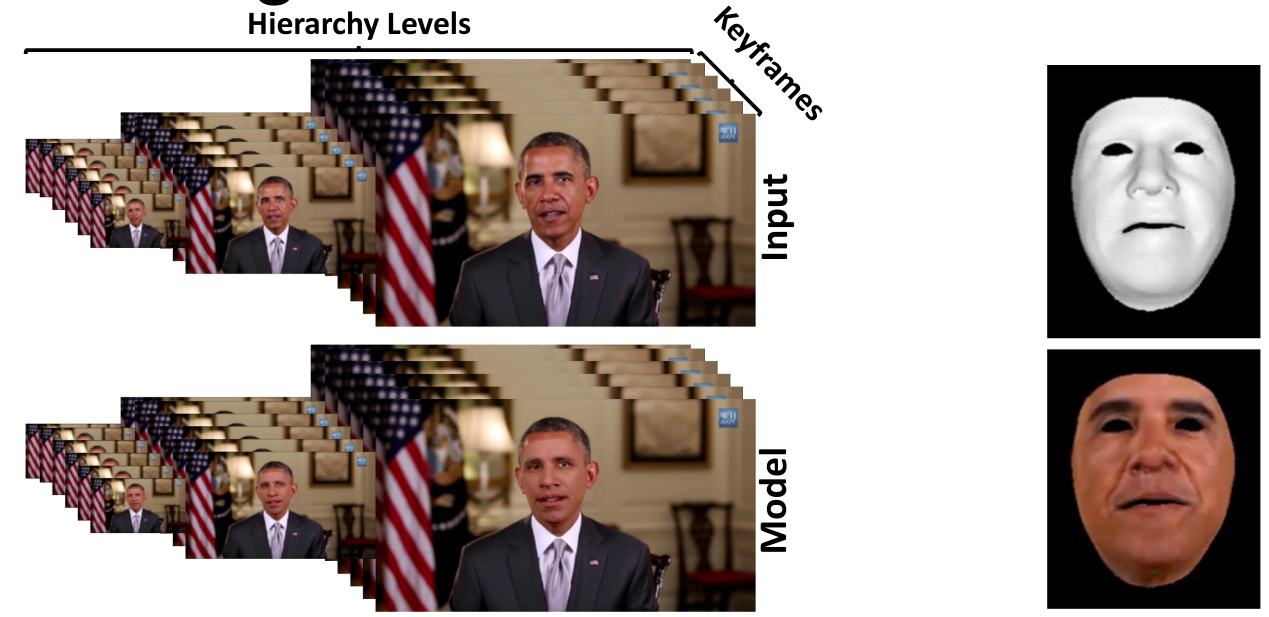
\includegraphics[width=0.5\textwidth]{images/nrmbb.png}
\end{center}
\caption{Use of sets of keyframes to compute a face with the Face2Face method \citep{Thies2016}}
\end{figure}

Once the tracked face is modeled, the parameters of the tracking can be modified in real-time with imported parameters from a source face, i.e. to perform facial feature transfers and reenactments. This phase relies on two steps: an expression transfer, and a mouth retrieval (see Figure 2). This is done per frame in a video. The geometry of the target face is modified to fit the source's face parameters while the target's face texture is kept.

The mouth retrieval phase is used to fill the inside of a mouth during reenactment and relies on the use of a database computed from the target's video (See Figure 6). The new face features and the interior of the mouth are composed together into an end result (the mouth interior is retrieved via k-nearest neighbors between the source's mouth and the created database).

\begin{figure}[H]
\begin{center}
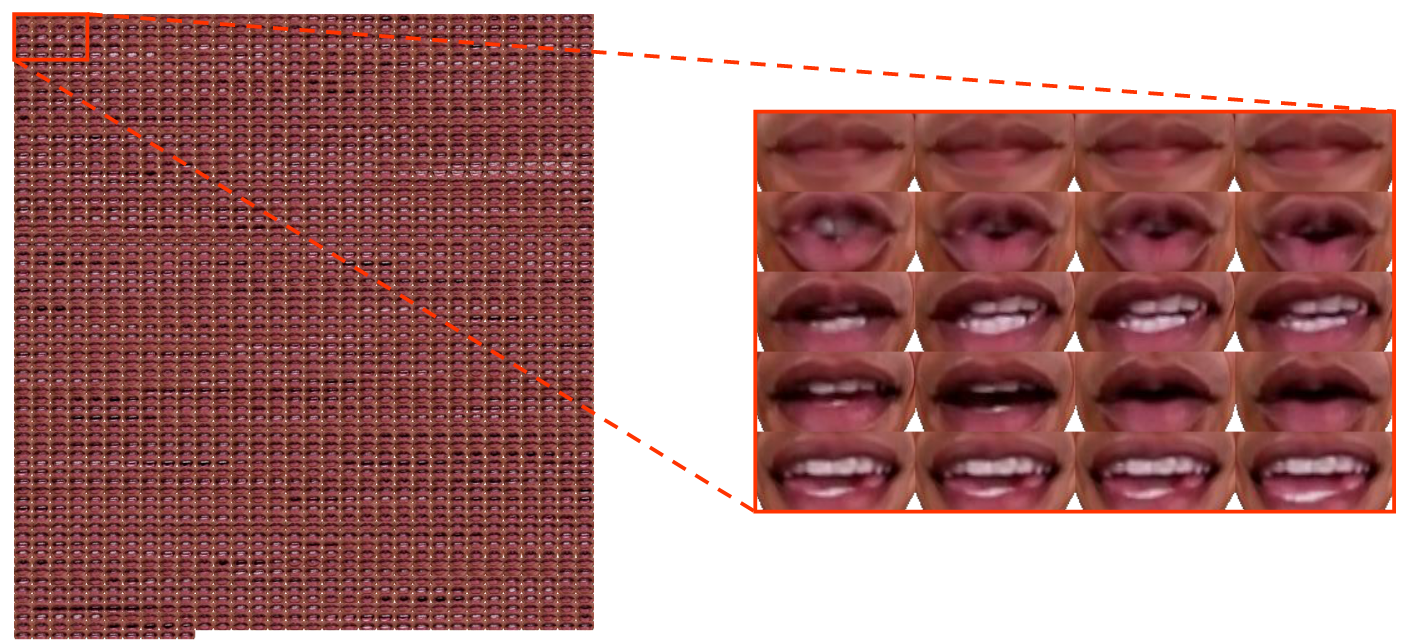
\includegraphics[width=0.5\textwidth]{images/mouth_database.png}
\end{center}
\caption{Mouth database being produced with the Face2Face method \citep{Thies2016}}
\end{figure}

The method is limited in some regards, assuming a smooth illumination, the absence of face occlusion (e.g. a hand, mask, etc.), and a training phase with regards to the computing of a mouth database. Furthermore, personal details are lost in the process, such as wrinkles.

\subsubsection{Graphics-based methods: FaceSwap}

Similar to Face2Face, the FaceSwap methods relies on detecting facial features, or landmarks, to identify the face region in a source video. Given a pre-constructed three-dimensional facial template, the source faces is blended in and projected onto a target image where facial features have also been detected. 

The projection relies on minimizing the difference between the source template and the target. Once the transfer has been performed and blended in the target video, the image is color-corrected.

\subsubsection{Learning-based methods: DeepFakes}

The DeepFakes method relies on learning the shape of a face from a source video and pasting it in a target video using an autoencoder setup. Two autoencoders are typically used on source and target images or videos, where feature maps of the corresponding cropped faces are learned. 


With such a setup (see Figure 7), and once the training phase is done, the encoder of the source-processing autoencoder and the decoder of the target-processing autoencoder are combined. As such, the context (feature map) of the source video or image is used to reconstruct the original data of the target video or image.

\begin{figure}[H]
\begin{center}
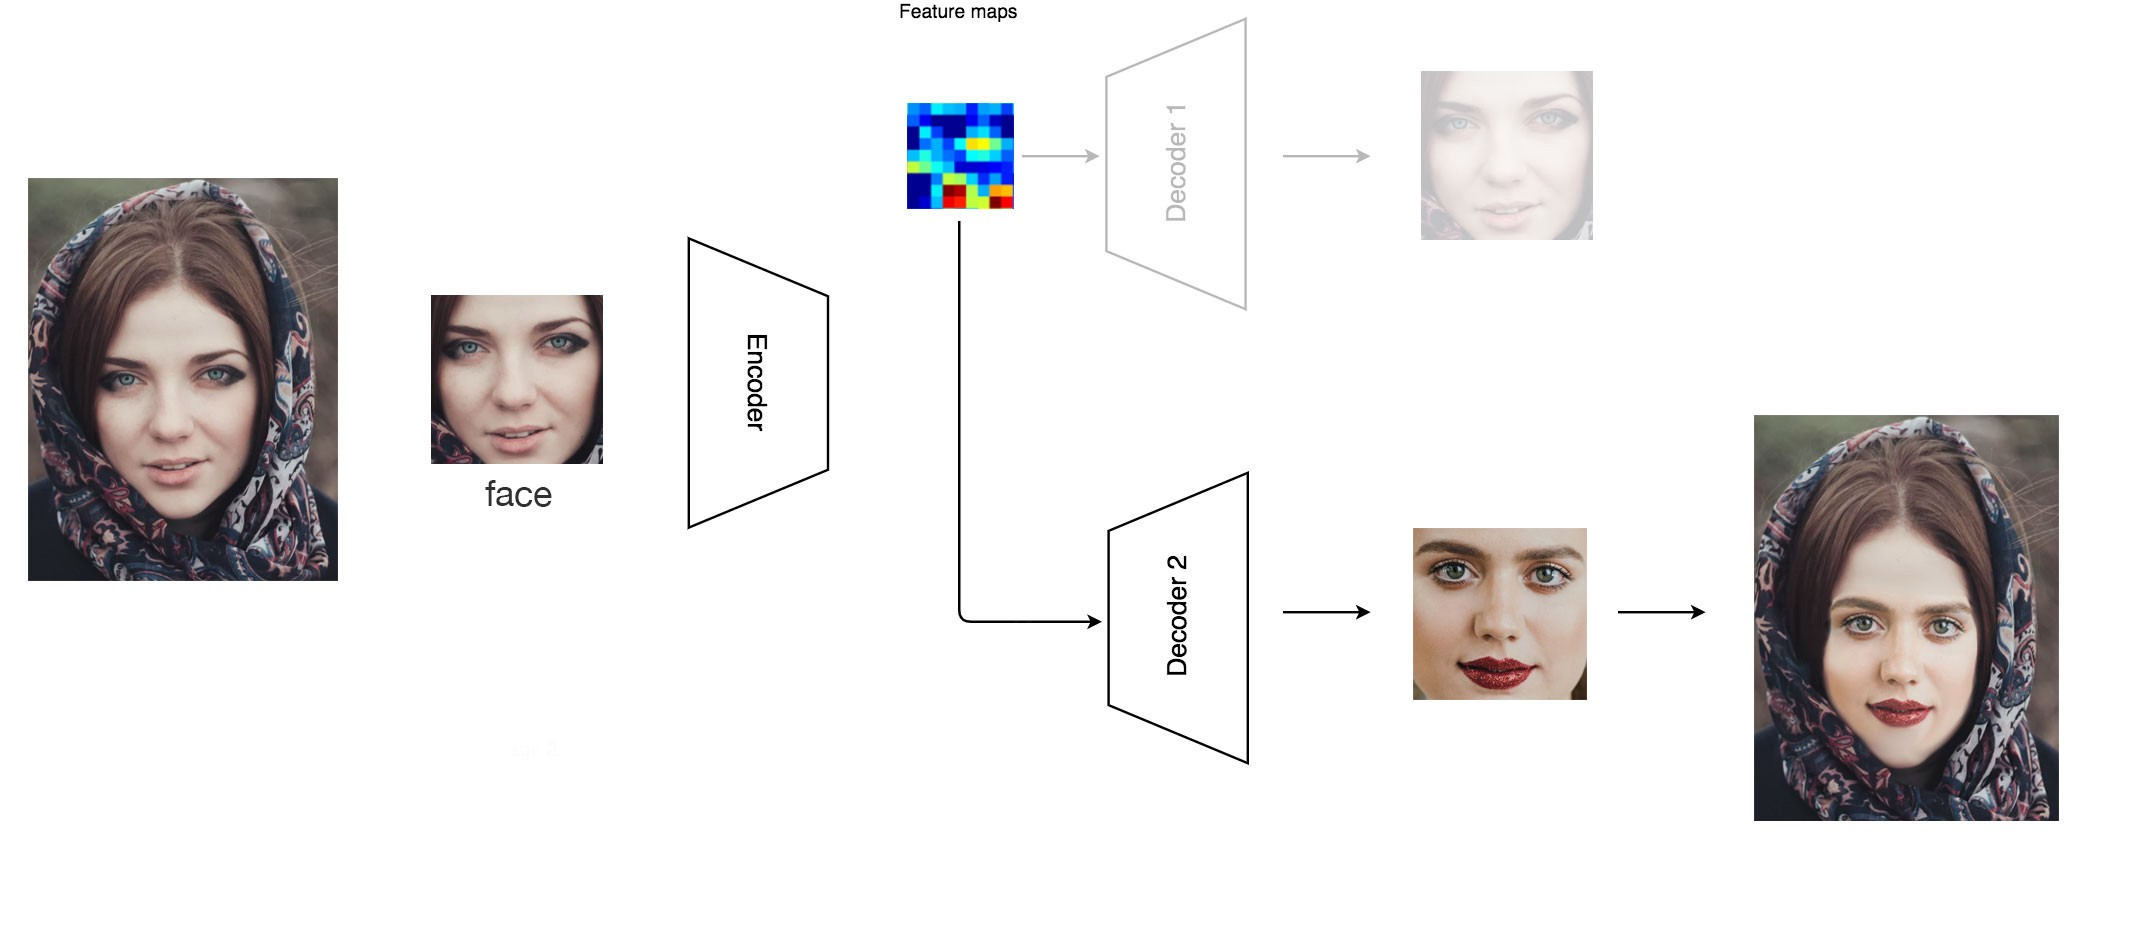
\includegraphics[width=0.9\textwidth]{images/deepfake.jpeg}
\end{center}
\caption{Autoencoding process to produce DeepFakes images \citep{hui}}
\end{figure}


A blending/cleaning step is then performed, yielding a DeepFake content.

\subsubsection{Learning-based methods: NeuralTextures}

NeuralTextures is a learning-based methods where a neural network is used to learn facial renderings in a generative adversarial setting. Generative Adversarial Neural networks are a type of unsupervised machine learning process. GAN methodology relies on two competing models that competes against each other in order to retrieve and copy variations in a dataset. They are called discriminator and generator networks.

Usually the discriminator and generator are both convolutional neural networks. The problem set by a GAN is that the generator tries to maximize the discriminator's error rate while the discriminator tries to minimize it. This result in an adversarial setup that gives the method its namesake. 

In the case of image forgery, a generator networks will try to learn to produce fake images (based on a random noise vector) which will be tested by the discriminator network for authenticity. The discriminator is trained on a set of real images plus the fake images created by the generator while the generator is trained on the binary feedback of the discriminator (See Figure 8, \cite{silva}). 

\begin{figure}[H]
\begin{center}
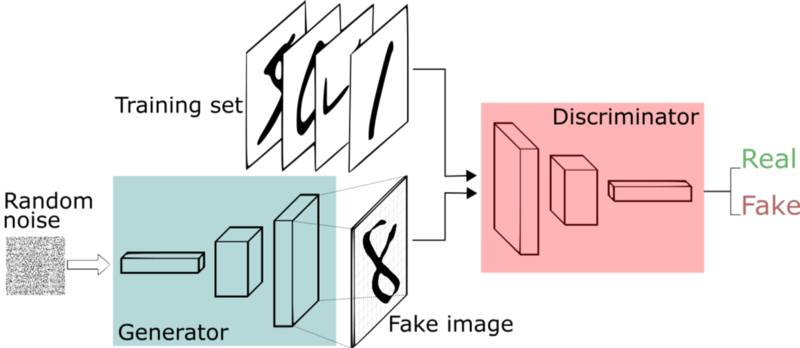
\includegraphics[width=0.7\textwidth]{images/GAN.png}
\end{center}
\caption{Generic representation of a GAN network trying to generate fake digit pictures based on the MNIST dataset \citep{silva}}
\end{figure}

In the case of NeuralTextures used in the paper, the method relies on the graphics-based method Face2Face in order to track and generate facial features besides the mouth area. The mouth area is generated using the GAN approach instead. The goal is to reduce the computational needs of the method.

\subsection{Forgery detection methods}

The team identified two types of forgery detection methods:
\begin{itemize}
    \item Expert-crafted steganographic features (hypothetical-deductive process)
    \item Learned features (inductive process)
\end{itemize}

However, both may target the same sets of evidence and hints in order to distinguish a forgery from a real image (see Table 2).

\begin{table}[h!]
\centering
\begin{tabular}{ |p{8.5cm}|p{4cm}|  }
 \hline
 \multicolumn{2}{|c|}{Generic artifacts} \\
 \hline
 \textbf{Type} & \textbf{Papers} \\
 \hline
 Dropped, duplicated frames & \cite{8014971} \\
 Interpolation & \cite{7869361} \\
 Copy-move (\footnotesize{part of an image is reused/copied to another part}) & \cite{8288661} \\
 Chroma-key (\footnotesize{Blending of different videos together such as foreground and background}) & \cite{8296533} \\
 \hline
 \multicolumn{2}{|c|}{Face artifacts} \\
 \hline
 \textbf{Type} & \textbf{Papers} \\
 \hline
 Computer graphics & \cite{8267647} \\
 Morphed face & \cite{8014962} \\
 Face splicing & \cite{7349174} \\
 Face swapping & \cite{8014963} \\
 Eye blinks & \cite{8630787} \\
 color/texture/shape cues & \cite{7349174} \\
 DeepFakes & \cite{8639163} \\
 \hline
\end{tabular}
\caption{State-of-the-art of face manipulation techniques}
\end{table}

Most modern forensics methods rely on convolutional neural networks to perform detection. They show "impressive results" but may be lacking robustness in the presence of common, practical cases such as resizing and compression -- common operations on online platforms. 

\subsection{Datasets available}

Historically, image forensics datasets were the result of "significant manual efforts under controlled conditions". The goal was to generate sets of images where specific forgery artifacts would manifest. Video footage was rarely addressed. Examples are displayed in Table 3.

\begin{table}[h!]
\centering
\begin{tabular}{ | p{4.5cm} | p{4.5cm} | p{4cm} |  }
 \hline
 \textbf{Dataset name} & \textbf{Content} & \textbf{Paper} \\
 \hline
 MICC\_F2000 & 700 images & \cite{5734842} \\
 Wild Web Dataset & 90 real cases & \cite{7169839} \\
 Realistic Tampering & 220 images & \cite{7776959} \\
 DeepFakes & 620 videos from 43 subjects & \cite{korshunov2018deepfakes} \\
 NIST & 50,000 images, 500 videos & \cite{8638296} \\
 \hline
\end{tabular}
\caption{Examples of classical image forensics datasets}
\end{table}

\section{The authors' motivations}

In this context, the paper's team (Andreas Rössler, Davide Cozzolino, Luisa Verdoliva, Christian Riess, Justus Thies, and Matthias Nießner) wished to push the literature on the topic of forgery detection and computer vision overall. As such, the authors wanted to contribute in four different aspects to the field:
\begin{itemize}
    \item A realistic, automated benchmark for future forgery detection techniques
    \item A robust assessment of the currently available detection methods
    \item A large scale, industry-shaping dataset
    \item A new, state-of-the-art method for detecting facial feature doctoring
\end{itemize}

\section{The paper's proposed approach}

\subsection{Proposing a new state-of-the-art dataset: FaceForensics++}

The FaceForensics++ datasets aims to cover realistic scenarios: "videos from the wild, manipulated and compressed with different quality levels". To this end, the paper's author proposed a new, state-of-the-art dataset that is an order of magnitude bigger than previous iterations (more than 1.8 million images drawn from c. 4000 fake videos, see Table 4).

\begin{table}[h!]
\centering
\begin{tabular}{ |p{4cm}|p{2.5cm}|p{2.5cm}| p{2.5cm}| }
 \hline
 \textbf{Methods} & \textbf{Train} & \textbf{Validation} & \textbf{Test} \\
 \hline
 Pristine & 366,847 & 68,511 & 73,770 \\
 Face2Face & 366,843 & 68,511 & 73,770 \\
 FaceSwap & 291,434 & 54,618 & 59,640 \\
 DeepFakes & 366,835 & 68,506 & 73,768 \\
 NeuralTextures & 291,834 & 54,630 & 59,672 \\
 \hline
\end{tabular}
\caption{Number of images per manipulation method}
\end{table}

The goal of such a dataset is to enable the training of newer, better forensic tools to apprehend the new forgery methods that deep-learning has notably enabled. 

In order to construct this dataset, the authors relied on videos from the YouTube platform (YouTube-8m dataset, videos with the tags "face", "newscaster", "newsprogram", "interview", "[video] blog"), manually screened to ensure the current forgery method will work (see Figure 9). 

\begin{figure}[H]
\begin{center}
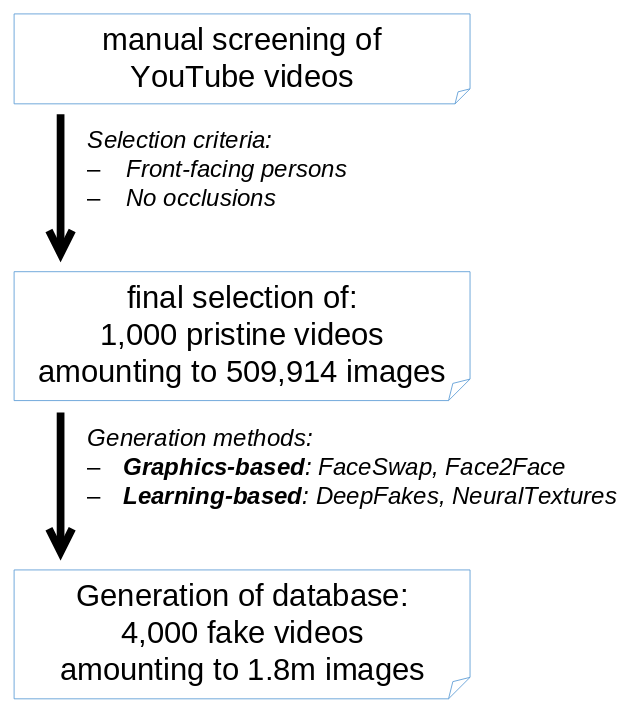
\includegraphics[width=0.5\textwidth]{images/process.png}
\end{center}
\caption{Dataset generation process}
\end{figure}

A further selection criteria focuses on diversity of format, for example relating to video quality, to emulate the varied content that can be found online (see Figure 10). The dataset construction relies on the 4 state-of-the-art methods previously presented: FaceSwap, Face2Face, DeepFakes, and NeuralTextures.

Whereas the DeepFakes manipulates each frame in a target video, the FaceSwap and NeuralTextures methods doctor the minimum amount of frames across both source and target videos. Finally, Face2Face maps all expressions of the source video onto the target video.

\begin{figure}[H]
\begin{center}
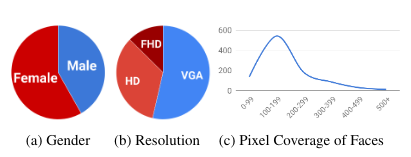
\includegraphics[width=0.5\textwidth]{images/stats.png}
\end{center}
\caption{Statistics of the FaceForensics++ sequences \citep{DBLP:journals/corr/abs-1803-09179}. VGA denotes 480p, HD denotes 720p, and FHD denotes 1080p resolution of the videos. The graph (c) shows the number of sequences (y-axis) with given bounding box pixel height (x-axis).}
\end{figure}


\subsection{Formalizing the problem of forgrey detection}

The authors represent the problem of forgery detection as a per-frame binary classification with regards to video forensics. Based on the produced database, the authors split the data between training, validation and test sets with the following ratios: 72\%, 14\%, 14\%.

In order to formalize the problem, the authors first performed a human trial with computer science students in order to construct a human baseline for the detection of forgeries. Given a set times to classify a random set of fake and pristine images, humans struggled to classify images produced by the Face2Face and NeuralTexture methods. 

Once the human baseline is constructed, the authors tested a thorough selection of learning-based and steganalytic (hand-crafted features followed by a SVM) methods. Compared to the humans, who were presented full pictures, the automatic forgery detection methods were presented images that underwent a first step of processing, called "domain-specific knowledge", where the images have been conservatively cropped to the face region using the face tracking method proposed by \cite{thies2020face2face}.

Overall, the automatic methods covered by the paper are listed in Table 5. Each was trained using the hyperparameters listed in Table 6 using the Adam optimizer with default values. The transfer learning process used for the XceptionNet model followed two phases: a first 3-epoch training where only the last, newly-inserted fully connected layer is trained, then a 15-epoch training phase where all the weights are trained.

Furthermore, the model were trained and tested in two given situation, either on one set of data, or on all four at once.

\begin{table}[h!]
\centering
\begin{tabular}{ |p{2cm}|p{7cm}|p{4cm}| }
 \hline
 \textbf{Type} & \textbf{Method} & \textbf{Paper} \\
 \hline
 Steganalysis & Hand-crafted processed followed by SVM & \cite{6197267} \\
 Learned & Steganalysis features of the previous method as a starting point to a CNN & \cite{10.1145/3082031.3083247} \\
  & Constrained CNN & \cite{8335799} \\
  & Stats-2L CNN & \cite{8267647} \\
  & MesoInception-4 (based on InceptionNet) & \cite{8630761} \\
  & XceptionNet (Transfer Learning) & \cite{8099678} \\
 \hline
\end{tabular}
\caption{Methods covered in the paper}
\end{table}

\begin{table}[h!]
\centering
\begin{tabular}{ |p{4cm}|p{3cm}|p{3cm}|}
 \hline
 \textbf{Model} & \textbf{Learning rate} & \textbf{Batch size} \\
 \hline
 \cite{10.1145/3082031.3083247} & $10^{-5}$ & $16$ \\
 \cite{8335799} & $10^{-5}$ & $64$ \\
 \cite{8267647} & $10^{-4}$ & $64$ \\
 \cite{8630761} & $10^{-3}$ & $76$ \\
 \cite{8099678} & $0.0002$ & $32$ \\
 \hline
\end{tabular}
\caption{Method hyperparameters}
\end{table}

For computing accuracy of the learning-based methods, the authors implemented an averaging process over 100 images per video, during validation and testing, and 270 images per video during training. Finally, they implemented an early-stopping heuristic where accuracy is evaluated 10 times during validation. If no improvement is recorded, the training stops. The imbalance in the dataset (more fakes than pristine videos) is dealt by weight-balancing the training images.

\subsection{Proposing a benchmark}
 
Using a further 1,000 pristine videos from YouTube as a baseline, the authors created a public benchmark for researchers to use to test their forgery detection solution.

Each participant in the benchmark (limited to once every two weeks) is provided one thousand images yielded from the dataset (either pristine or forged using one of the four previously presented methods) to analyze.

The goal of the benchmark is to push the research in forgery detection, but also offer a comparison metric between future research. In that sense, the FaceForensics++ paper is a seminal one.

\begin{figure}[H]
\begin{center}
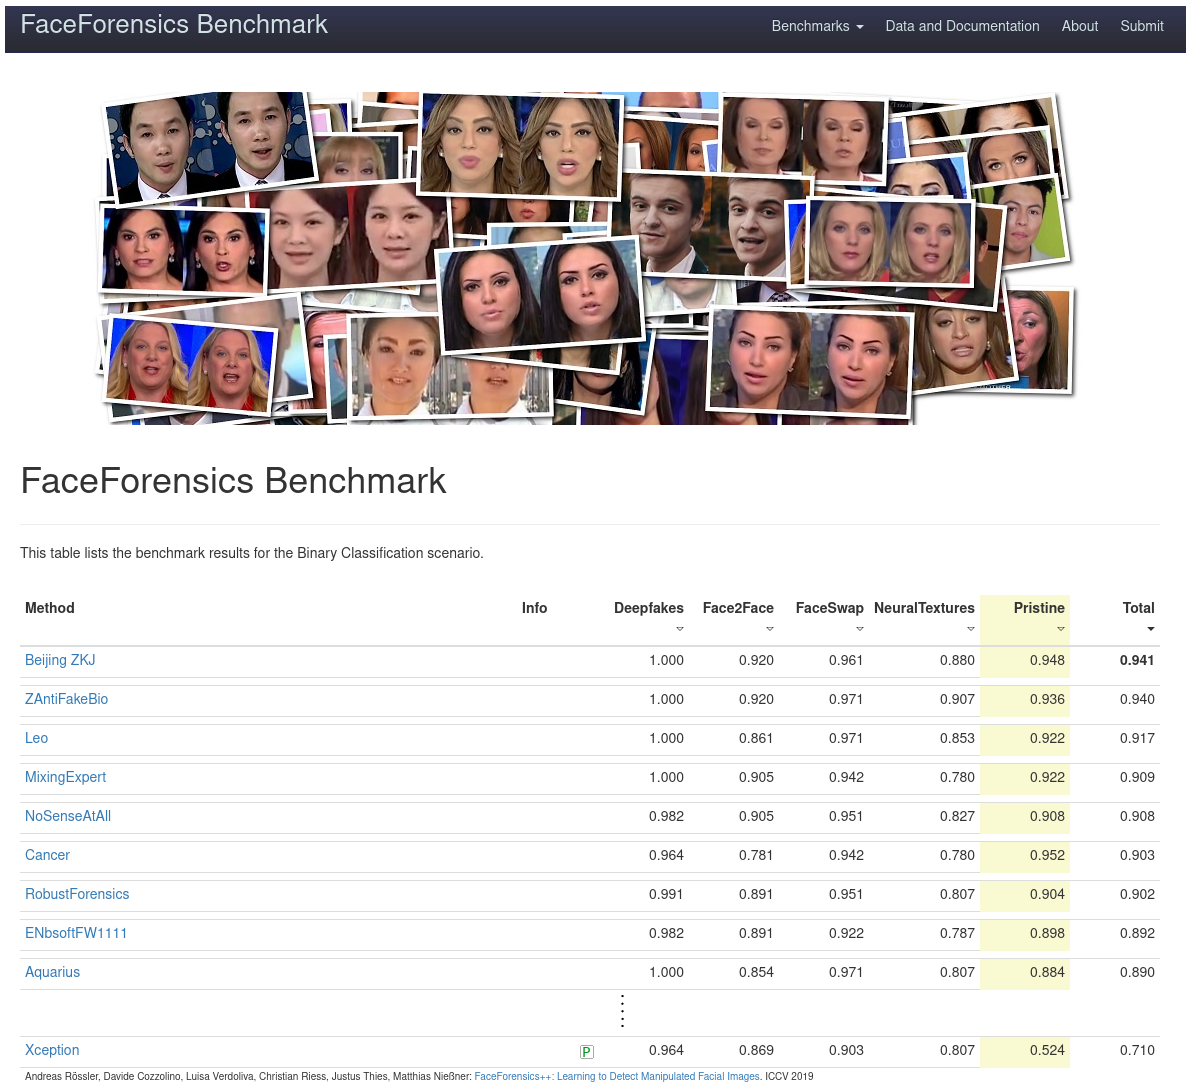
\includegraphics[width=\textwidth]{images/benchmark.png}
\end{center}
\caption{FaceForensics++ Benchmark Leaderboard}
\end{figure}
 
\section{Results, performance, and limitations}

The second result from the paper is that forgery detection methods perform best on raw input -- increasing levels of compression lead to downgraded detection performance. Neural networks are more resilient to compression.

When combined with domain-specific knowledge (face isolation), the neural network XceptionNet yields the best performance on all tests.

NeuralTextures is the most challenging doctoring method to detect. DeepFakes, despite being a neural network method is relatively easily detectable as the method relies on a post-processing step that yields detectable artifacts.

Results per architecture/methods are listed in Figure 13 and 14. It is interesting to note that computer detection methods perform better than human at detecting forgeries (see Figure 12).

\begin{figure}[H]
\begin{center}
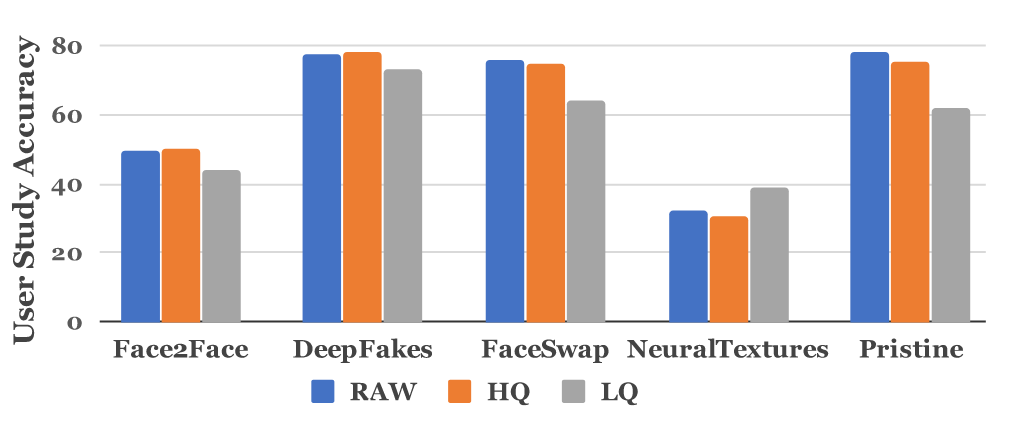
\includegraphics[width=0.8\textwidth]{images/human.png}
\end{center}
\caption{Human baseline, accuracy of forged pictures from the FaceForensics++ dataset}
\end{figure}

\begin{figure}[H]
\begin{center}
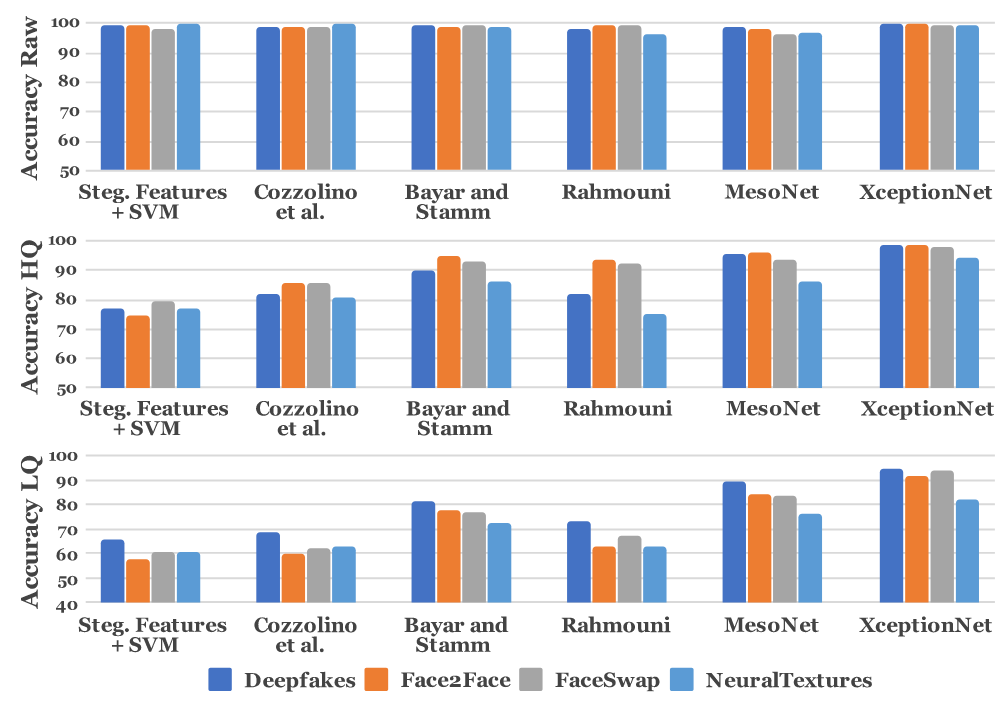
\includegraphics[width=0.8\textwidth]{images/single.png}
\end{center}
\caption{Architecture results, average accuracy of forged pictures from the FaceForensics++ dataset when trained on each manipulation methods separately}
\end{figure}

\begin{figure}[H]
\begin{center}
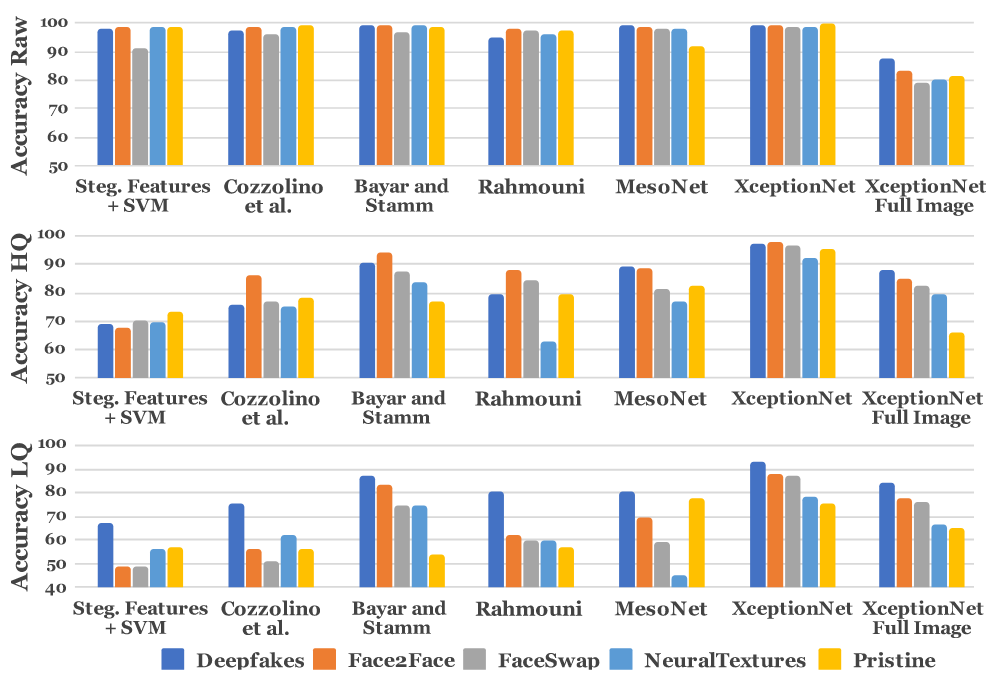
\includegraphics[width=0.8\textwidth]{images/multi.png}
\end{center}
\caption{Architecture results, average accuracy of forged pictures from the FaceForensics++ dataset when trained on all manipulation methods at once}
\end{figure}

The main limitations of the current image forgery methods as at the publication of the paper and still today is the need for source and target videos to be front-facing, single-shot, without occlusions. The benchmark and most doctoring and detection methods revolves around producing and detecting videos and images that follow those principle. Furthermore, the detection relies on first singling out faces within a pictures.

The development of doctoring methods that can overcome that limitation would put into question existing papers, datasets, and benchmarks, including the one proposed by the paper.

\section{Future directions}

styleGAN https://en.wikipedia.org/wiki/StyleGAN

https://paperswithcode.com/paper/video-face-manipulation-detection-through

https://paperswithcode.com/paper/mantra-net-manipulation-tracing-network-for

https://paperswithcode.com/dataset/dfdc

\section{Reimplementing the XceptionNet}

\section{Conclusion}

Though limited in some extent, the ability to produce image forgeries has exploded over the past few years. The social, economic and political risks forgeries raise leads to an ever-increasing risk to detect them. As such, FaceForensics++ is a seminal paper and dataset in the area of computer vision and specifically the detection of forgeries produced by the current state-of-the-art.

\clearpage

\bibliography{iclr2021_conference}
\bibliographystyle{iclr2021_conference}

\clearpage
\appendix

\section*{Appendix A - Constrained CNN}

Presented in 2018 by \cite{8335799}, a constrained CNN is a CNN method that uses a new type of layer at its start. The goal is to help the network learn not an image's content but manipulation traces. This new layer is trained in a similar fashion as a normal CNN, expect that it undergoes a normalization step where the middle weight of the filter (in a 3x3 instance case) is set to -1 while the surrounding weights are normalized to sum up to 1.

\begin{figure}[H]
\begin{center}
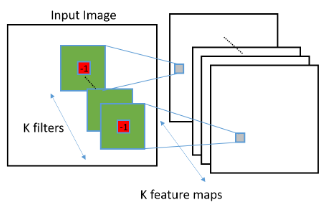
\includegraphics[width=0.5\textwidth]{images/conslayer.png}
\end{center}
\caption{Constrained CNN layer. The middle weight is set to 1, and the surrounding ones normalized to sum up to 1}
\end{figure}

\begin{figure}[H]
\begin{center}
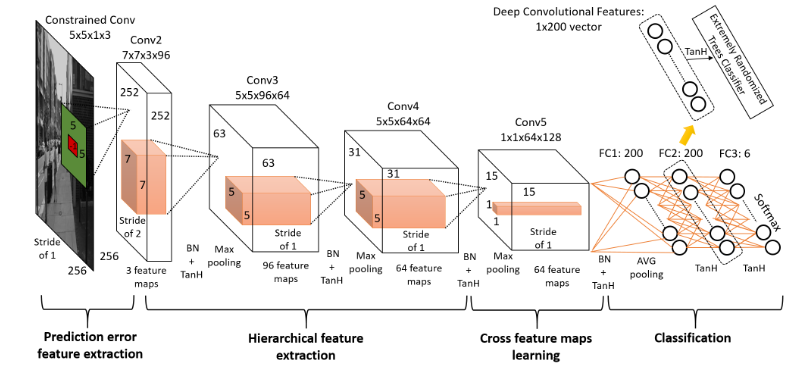
\includegraphics[width=\textwidth]{images/consCNN.png}
\end{center}
\caption{Constrained CNN as proposed by \cite{8335799}}
\end{figure}

\end{document}